\chapter{Arrays of Objects}

During the next three chapters, we will develop programs that work with playing cards and decks of cards.
Here is an outline of the road ahead:

\begin{itemize}

\item In this chapter, we define a \java{Card} class and write methods that work with cards and arrays of cards.

\item In Chapter~\ref{deck}, we define a \java{Deck} class that encapsulates an array of cards, and we write methods that operate on decks.

\item In Chapter~\ref{eights}, we introduce a way to define new classes that extend existing classes.
Then we use \java{Card} and \java{Deck} to implement the game {\it Crazy Eights}.

\end{itemize}

%Although we will see several versions of the same code, the main advantage of proceeding this way is that the explanations will be smoother.
%It may help you to create a {\tt Card.java} file and paste in the examples as we go.

%The code for this chapter is in the directory {\tt ch12} in the repository for this book.
%Instructions for downloading the repository are on page~\pageref{code}.
%Before proceeding, we recommend that you preview the {\tt Card.java} file.

\index{rank}
\index{suit}

There are 52 cards in a standard deck.
Each card belongs to one of four suits and one of 13 ranks.
The suits are Clubs, Diamonds, Hearts, and Spades.
The ranks are Ace, 2, 3, 4, 5, 6, 7, 8, 9, 10, Jack, Queen, and King.

If you are unfamiliar with traditional playing cards, now would be a good time to get a deck or read through \url{https://en.wikipedia.org/wiki/Standard_52-card_deck}.


\section{Card Objects}

\index{Card}
\index{class!Card}

If we want to define a class to represent a playing card, it is pretty clear what the instance variables should be: \java{rank} and \java{suit}.
It is not as obvious what types they should be.

One possibility is a \java{String} containing things like \java{"Spade"} for suits and \java{"Queen"} for ranks.
A problem with this choice is that it would not be easy to compare cards to see which had a higher rank or suit.

\index{encode}
\index{map to}

An alternative is to use integers to {\bf encode} the ranks and suits.
By encode, we {\em don't} mean to encrypt or translate into a secret code.
We mean to define a mapping between a sequence of numbers and the things we want to represent.

Here is a mapping for suits:

\begin{tabular}{l c l}
Clubs & $\mapsto$ & 0 \\
Diamonds & $\mapsto$ & 1 \\
Hearts & $\mapsto$ & 2 \\
Spades & $\mapsto$ & 3
\end{tabular}

% DW suggests using constants for CLUBS, DIAMONDS, etc.
% ABD thinks good idea, but will require changes in the code and book.
% CSM: an object-oriented solution would use enums instead of constants

We use the mathematical symbol $\mapsto$ to make it clear that these mappings are not part of the program.
They are part of the program design, but they never appear explicitly in the code.

Each of the numerical ranks (2 through 10) maps to the corresponding integer.
For the face cards, we can use:

\begin{tabular}{l c l}
Ace & $\mapsto$ & 1 \\
Jack & $\mapsto$ & 11 \\
Queen & $\mapsto$ & 12 \\
King & $\mapsto$ & 13 \\
\end{tabular}

With this encoding, the class definition for the \java{Card} type looks like this:

\begin{code}
public class Card {
    private int rank;
    private int suit;

    public Card(int rank, int suit) {
        this.rank = rank;
        this.suit = suit;
    }
}
\end{code}

\index{constructor}

The instance variables are \java{private}: we can access them from inside this class, but not from other classes.

The constructor takes a parameter for each instance variable.
To create a \java{Card} object, we use the \java{new} operator:

\begin{code}
Card threeOfClubs = new Card(3, 0);
\end{code}

%The second argument, \java{0} represents the suit Clubs.
The result is a reference to a \java{Card} that represents the ``3 of Clubs''.


\section{Card toString}

\index{print!Card}

When you create a new class, the first step is to declare the instance variables and write constructors.
A good next step is to write \java{toString}, which is useful for debugging and incremental development.

\index{string!array of}
\index{array!of strings}

To display \java{Card} objects in a way that humans can read easily, we need to ``decode'' the integer values as words.
A natural way to do that is with an array of \java{String}s.
For example, we can create the array like this:

\begin{code}
String[] suits = new String[4];
\end{code}

And then assign values to the elements:

\begin{code}
suits[0] = "Clubs";
suits[1] = "Diamonds";
suits[2] = "Hearts";
suits[3] = "Spades";
\end{code}

Or we can create the array and initialize the elements at the same time, as we saw in Section~\ref{printarray}:

\begin{code}
String[] suits = {"Clubs", "Diamonds", "Hearts", "Spades"};
\end{code}

\index{memory diagram}
\index{diagram!memory}
\index{reference}
\index{string!reference to}

The memory diagram in Figure~\ref{fig.stringarray} shows the result.
Each element of the array is a reference to a \java{String}.

\begin{figure}[!ht]
\begin{center}
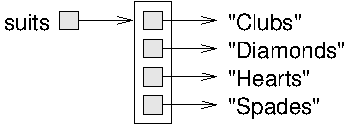
\includegraphics{figs/stringarray.pdf}
\caption{Memory diagram of an array of strings.}
\label{fig.stringarray}
\end{center}
\end{figure}

We also need an array to decode the ranks:

\begin{code}
String[] ranks = {null, "Ace", "2", "3", "4", "5", "6",
           "7", "8", "9", "10", "Jack", "Queen", "King"};
\end{code}

The zeroth element should never be used, because the only valid ranks are 1--13.
We set it to \java{null} to indicate an unused element.

Using these arrays, we can create a meaningful \java{String} using \java{suit} and \java{rank} as indexes.

\begin{code}
String s = ranks[this.rank] + " of " + suits[this.suit];
\end{code}

The expression \java{ranks[this.rank]} means ``use the instance variable \java{rank} from \java{this} object as an index into the array \java{ranks}.''
We select the string for \java{this.suit} in a similar way.

Now we can wrap all the previous code in a \java{toString} method.

\begin{code}
public String toString() {
    String[] ranks = {null, "Ace", "2", "3", "4", "5", "6",
               "7", "8", "9", "10", "Jack", "Queen", "King"};
    String[] suits = {"Clubs", "Diamonds", "Hearts", "Spades"};
    String s = ranks[this.rank] + " of " + suits[this.suit];
    return s;
}
\end{code}

When we display a card, \java{println} automatically calls \java{toString}.
The output of the following code is {\tt Jack of Diamonds}.

\begin{code}
Card card = new Card(11, 1);
System.out.println(card);
\end{code}


\section{Class Variables}
\label{classvar}

\index{class variable}

So far we have seen local variables, which are declared inside a method, and instance variables, which are declared in a class definition, usually before the method definitions.
Now it's time to learn about {\bf class variables}.
They are shared across all instances of the class.

%Local variables are created when a method is invoked, and their space is reclaimed when the method ends.
%Instance variables are created when you construct an object and reclaimed when the object is garbage-collected.

\index{static}
\index{variable!static}

Like instance variables, class variables are defined in a class definition, before the method definitions.
But they are identified by the keyword \java{static}.
Here is a version of \java{Card} where \java{RANKS} and \java{SUITS} are defined as class variables:

\begin{code}
public class Card {

    public static final String[] RANKS = {
        null, "Ace", "2", "3", "4", "5", "6", "7",
        "8", "9", "10", "Jack", "Queen", "King"};

    public static final String[] SUITS = {
        "Clubs", "Diamonds", "Hearts", "Spades"};

    // instance variables and constructors go here

    public String toString() {
        return RANKS[this.rank] + " of " + SUITS[this.suit];
    }
}
\end{code}

\index{garbage collection}

Class variables are allocated when the program begins and persist until the program ends.
In contrast, instance variables like \java{rank} and \java{suit} are allocated when the program creates \java{new} objects, and they are deleted when the object is garbage-collected.

% ABD: Let's check whether garbage collection ends up before this.

\index{final}

%You can refer to a class variable from anywhere inside the class definition.
Class variables are often used to store constant values that are needed in several places.
In that case, they should also be declared as \java{final}.
Note that whether a variable is \java{static} or \java{final} involves two separate considerations:
\java{static} means the variable is {\em shared}, and \java{final} means the variable is {\em constant}.

Naming \java{static final} variables with capital letters is a common convention that makes it easier to recognize their role in the class.
In the \java{toString} method, we refer to \java{SUITS} and \java{RANKS} as if they were local variables, but we can tell that they are class variables.

One advantage of defining \java{SUITS} and \java{RANKS} as class variables is that they don't need to be created (and garbage-collected) every time \java{toString} is called.
They may also be needed in other methods and classes, so it's helpful to make them available everywhere.
Since the array variables are \java{final}, and the strings they reference are immutable, there is no danger in making them \java{public}.


\section{The compareTo Method}

\index{equivalent}

As we saw in Section~\ref{equals}, it's helpful to create an \java{equals} method to test whether two objects are equivalent.

\begin{code}
public boolean equals(Card that) {
    return this.rank == that.rank
        && this.suit == that.suit;
}
\end{code}

\index{operator!logical}
\index{logical operator}

It would also be nice to have a method for comparing cards, so we can tell if one is higher or lower than another.
For primitive types, we can use comparison operators like \java{<} and \java{>} to compare values.
But these operators don't work for object types.

For strings, Java provides a \java{compareTo} method, as we saw in Section~\ref{strcmp}.
We can write our own version of \java{compareTo} for the classes that we define, like we did for the \java{equals} method.
%Later we will use this method to sort a deck of cards.

\index{ordering}
\index{complete ordering}
\index{partial ordering}

Some types are ``totally ordered'', which means that you can compare any two values and tell which is bigger.
Integers and strings are totally ordered.
Other types are ``unordered'', which means that there is no meaningful way to say that one element is bigger than another.
In Java, the \java{boolean} type is unordered; if you try to compare \java{true < false}, you get a compiler error.

The set of playing cards is ``partially ordered'', which means that sometimes we can compare cards and sometimes not.
For example, we know that the 3 of Clubs is higher than the 2 of Clubs, and the 3 of Diamonds is higher than the 3 of Clubs.
But which is better, the 3 of Clubs or the 2 of Diamonds?
One has a higher rank, but the other has a higher suit.

\index{compareTo}

To make cards comparable, we have to decide which is more important: rank or suit.
The choice is arbitrary, and it might be different for different games.
But when you buy a new deck of cards, it comes sorted with all the Clubs together, followed by all the Diamonds, and so on.
So for now, let's say that suit is more important.
With that decided, we can write \java{compareTo} as follows:

\begin{code}
public int compareTo(Card that) {
    if (this.suit < that.suit) {
        return -1;
    }
    if (this.suit > that.suit) {
        return 1;
    }
    if (this.rank < that.rank) {
        return -1;
    }
    if (this.rank > that.rank) {
        return 1;
    }
    return 0;
}
\end{code}

\java{compareTo} returns \java{-1} if \java{this} is a lower card, \java{+1} if \java{this} is a higher card, and \java{0} if \java{this} and \java{that} are equivalent.
It compares suits first.
If the suits are the same, it compares ranks.
If the ranks are also the same, it returns 0.


\section{Cards are Immutable}

The instance variables of \java{Card} are \java{private}, so they can't be accessed from other classes.
We can provide getters to allow other classes to read the \java{rank} and \java{suit} values:

\begin{code}
public int getRank() {
    return this.rank;
}

public int getSuit() {
    return this.suit;
}
\end{code}

\index{immutable}

Whether or not to provide setters is a design decision.
If we did, cards would be mutable, so you could transform one card into another.
That is probably not a feature we want, and in general, mutable objects are more error-prone.
So it might be better to make cards immutable.
To do that, all we have to do is {\em not} provide any modifier methods (including setters).

\index{final}

That's easy enough, but it is not foolproof, because a fool might come along later and add a modifier.
We can prevent that possibility by declaring the instance variables \java{final}:

\begin{code}
public class Card {
    private final int rank;
    private final int suit;

    ...
}
\end{code}

You can still assign values to these variables inside a constructor.
But if someone writes a method that tries to modify these variables, they'll get a compiler error.
This kind of safeguard helps prevent future mistakes and hours of debugging.


\section{Arrays of Cards}
\label{cardarray}

%\index{composition}

%By now we have seen several examples of composition; that is, the ability to combine language features in a variety of arrangements.
%One of the first examples we saw was using a method invocation as part of an expression.
%Another example is the nested structure of statements: you can put an \java{if} statement within a \java{while} loop, or within another \java{if} statement, etc.

%Having seen this pattern, and having learned about arrays and objects, you should not be surprised to learn that you can make arrays of objects.
%And you can define objects with arrays as instance variables; you can make arrays that contain arrays; you can define objects that contain objects, and so on.

\index{array!of objects}
\index{object!array of}

Just as you can create an array of \java{String} objects, you can create an array of \java{Card} objects.
The following statement creates an array of 52 cards.
Figure~\ref{fig.cardarray} shows the memory diagram for this array.

\begin{code}
Card[] cards = new Card[52];
\end{code}

\begin{figure}[!ht]
\begin{center}
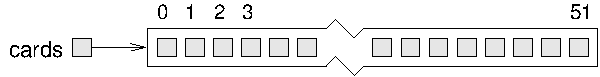
\includegraphics{figs/cardarray.pdf}
\caption{Memory diagram of an unpopulated \java{Card} array.}
\label{fig.cardarray}
\end{center}
\end{figure}

% ABD: I might redraw this to use dashed lines instead of zig-zag to indicate the elided part of the array.

\index{null}

Although we call it an ``array of cards'', the array contains {\em references} to cards; it does not contain the \java{Card} objects themselves.
Initially the references are all \java{null}.

Even so, you can access the elements of the array in the usual way:

\begin{code}
if (cards[0] == null) {
    System.out.println("No card yet!");
}
\end{code}

\index{exception!NullPointer}
\index{run-time error}

But if you try to access the instance variables of non-existent \java{Card} objects, you will get a \java{NullPointerException}.

\begin{code}
System.out.println(cards[0].rank);  // NullPointerException
\end{code}

\index{nesting}
\index{loop!nested}

That code won't work until we put cards in the array.
One way to populate the array is to write nested \java{for} loops:

\begin{code}
int index = 0;
for (int suit = 0; suit <= 3; suit++) {
    for (int rank = 1; rank <= 13; rank++) {
        cards[index] = new Card(rank, suit);
        index++;
    }
}
\end{code}

The outer loop iterates suits from 0 to 3.
For each suit, the inner loop iterates ranks from 1 to 13.
Since the outer loop runs 4 times, and the inner loop runs 13 times for each suit, the body is executed 52 times.

\index{index}

We use a separate variable \java{index} to keep track of where in the array the next card should go.
Figure~\ref{fig.cardarray2} shows what the array looks like after the first two cards have been created.

\begin{figure}[!ht]
\begin{center}
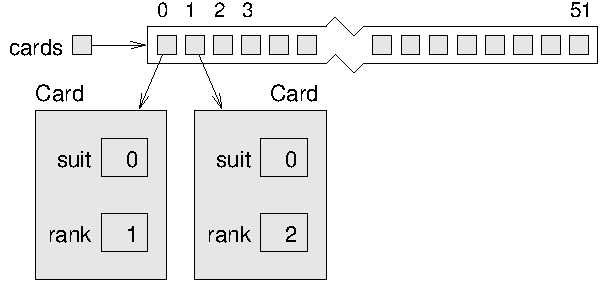
\includegraphics{figs/cardarray2.pdf}
\caption{Memory diagram of a \java{Card} array with two cards.}
\label{fig.cardarray2}
\end{center}
\end{figure}

\index{print!array}

When you work with arrays, it is convenient to have a method that displays the contents.
We have seen the pattern for traversing an array several times, so the following method should be familiar.

% ABD: Maybe add reference to where we introduced enhanced loops?

\begin{code}
public static void printDeck(Card[] cards) {
    for (Card card : cards) {
        System.out.println(card);
    }
}
\end{code}

%\begin{code}
%public static void printDeck(Card[] cards) {
%    for (int i = 0; i < cards.length; i++) {
%        System.out.println(cards[i]);
%    }
%}
%\end{code}

Since \java{cards} has type \java{Card[]}, pronounced ``card array'', an element of \java{cards} has type \java{Card}.
So \java{println} invokes the \java{toString} method in the \java{Card} class.

Then again, we don't have to write our own \java{printDeck} method.
The \java{Arrays} class provides a \java{toString} method that invokes \java{toString} on the elements of an array and concatenates the results.
To can invoke it like this:

\begin{code}
System.out.println(Arrays.toString(cards))
\end{code}


\section{Sequential Search}

\index{sequential search}

The next method we'll write is \java{search}, which takes an array of cards and a \java{Card} object as parameters.
It returns the index where the \java{Card} appears in the array, or \java{-1} if it doesn't.
This version of \java{search} uses the algorithm we saw in Section~\ref{traversal}, which is called {\bf sequential search}:

\index{traverse}
\index{loop!search}

\begin{code}
public static int search(Card[] cards, Card target) {
    for (int i = 0; i < cards.length; i++) {
        if (cards[i].equals(target)) {
            return i;
        }
    }
    return -1;
}
\end{code}

\index{statement!return}
\index{return!inside loop}

The method returns as soon as it discovers the card, which means we don't have to traverse the entire array if we find the target.
If we get to the end of the loop, we know the card is not in the array.

\index{efficiency}

If the cards in the array are not in order, there is no way to search faster than sequential search.
We have to look at every card, because otherwise we can't be certain the card we want is not there.
But if the cards are in order, we can use better algorithms.

Sequential search is relatively inefficient, especially for large arrays.
If you pay the price to keep the array sorted, finding elements becomes much easier.
%We will learn in the next chapter how to sort arrays.


\section{Binary Search}

% ABD:  I wonder if we need a different example.  I don't know how many students have looked up a word in a paper dictionary.

\index{binary search}

When you look for a word in a dictionary, you don't search page by page from front to back.
Since the words are in alphabetical order, you probably use a {\bf binary search} algorithm:

\begin{enumerate}

\item Start on a page near the middle of the dictionary.

\item Compare a word on the page to the word you are looking for.
If you find it, stop.

\item If the word on the page comes before the word you are looking for, flip to somewhere later in the dictionary and go to step 2.

\item If the word on the page comes after the word you are looking for, flip to somewhere earlier in the dictionary and go to step 2.

\end{enumerate}

This algorithm is much faster than sequential search, because it rules out half of the remaining words each time you make a comparison.
If at any point you find two adjacent words on the page, and your word comes between them, you can conclude that your word is not in the dictionary.

Getting back to the array of cards, we can write a faster version of \java{search} if we know the cards are in order:

\begin{code}
public static int binarySearch(Card[] cards, Card target) {
    int low = 0;
    int high = cards.length - 1;
    while (low <= high) {
        int mid = (low + high) / 2;                 // step 1
        int comp = cards[mid].compareTo(target);

        if (comp == 0) {                            // step 2
            return mid;
        } else if (comp < 0) {                      // step 3
            low = mid + 1;
        } else {                                    // step 4
            high = mid - 1;
        }
    }
    return -1;
}
\end{code}

First, we declare \java{low} and \java{high} variables to represent the range we are searching.
Initially we search the entire array, from \java{0} to \java{cards.length - 1}.

Inside the \java{while} loop, we repeat the four steps of binary search:

\begin{enumerate}

\item Choose an index between \java{low} and \java{high} -- call it \java{mid} -- and compare the card at \java{mid} to the target.

\item If you found the target, return its index (which is \java{mid}).

\item If the card at \java{mid} is lower than the target, search the range from \java{mid + 1} to \java{high}.

\item If the card at \java{mid} is higher than the target, search the range from \java{low} to \java{mid - 1}.

\end{enumerate}

If \java{low} exceeds \java{high}, there are no cards in the range, so we terminate the loop and return \java{-1}.

This algorithm only depends on the \java{compareTo} method of the object, so we can use this code with object type that provides \java{compareTo}.


\section{Tracing the Code}

\index{tracing}

To see how binary search works, it's helpful to add the following print statement at the beginning of the loop:

\begin{code}
System.out.println(low + ", " + high);
\end{code}

Using a sorted deck of cards, we can search for the ``Jack of Clubs'' like this:

\begin{code}
Card card = new Card(11, 0);
System.out.println(binarySearch(cards, card));
\end{code}

We expect to find this card at position 10 (since the ``Ace of Clubs'' is at position 0).
Here is the output of \java{binarySearch}:

\begin{stdout}
0, 51
0, 24
0, 11
6, 11
9, 11
10
\end{stdout}

You can see the range of cards shrinking as the \java{while} loop runs, until eventually index 10 is found.
If we search for a card that's not in the array, like \java{new Card(15, 1)} the ``15 of Diamonds'', we get the following:

\begin{stdout}
0, 51
26, 51
26, 37
26, 30
26, 27
-1
\end{stdout}

%\index{testing}
%\index{correctness}
%
%These tests don't prove that this program is correct.
%In fact, no amount of testing can {\em prove} that a program is correct.
%But looking at a few cases and examining the code, you might be able to convince yourself.

Each time through the loop, we cut the distance between \java{low} and \java{high} in half.
After $k$ iterations, the number of remaining cards is $52 / 2^k$.
To find the number of iterations it takes to complete, we set $52 / 2^k = 1$ and solve for $k$.
The result is $\log_2 52$, which is about 5.7.
So we might have to look at 5 or 6 cards, as opposed to all 52 if we did a sequential search.

More generally, if the array contains $n$ elements, binary search requires $\log_2 n$ comparisons, and sequential search requires $n$.
For large values of $n$, binary search is substantially faster.

% ABD: Following our discussion, I'm killing the recursive version of binarySearch.
% So this might be a good place for the scope discussion from
% Chapter 10.

%\section{Recursive Version}
%
%\index{recursion}
%
%Another way to implement binary search is with a recursive method.
%We take \java{low} and \java{high} as parameters, add a base case, and turn steps 3 and 4 into recursive invocations.
%%They indicate the segment of the array that should be searched (including both \java{low} and \java{high}).
%%Here's what that code looks like:
%
%\begin{code}
%public static int binarySearch(Card[] cards, Card target,
%                               int low, int high) {
%    if (high < low) {
%        return -1;
%    }
%    int mid = (low + high) / 2;                     // step 1
%    int comp = cards[mid].compareTo(target);
%
%    if (comp == 0) {                                // step 2
%        return mid;
%    } else if (comp < 0) {                          // step 3
%        return binarySearch(cards, target, mid + 1, high);
%    } else {                                        // step 4
%        return binarySearch(cards, target, low, mid - 1);
%    }
%}
%\end{code}
%
%Instead of a \java{while} loop, we have an \java{if} statement to terminate the recursion.
%%We call this \java{if} statement the base case.
%If \java{high} is less than \java{low}, there are no cards between them, and we conclude that the card is not in the array.
%
%\index{infinite recursion}
%\index{recursion!infinite}
%\index{StackOverflowError}
%\index{exception!StackOverflow}
%
%Two common errors in recursive methods are (1) forgetting to include a base case, and (2) writing the recursive call so that the base case is never reached.
%Either error causes infinite recursion and a \java{StackOverflowError}.


\section{Scope Revisited}

% TODO: If we decide to keep this here, it needs some revision for flow.

\index{scope}

In Section~\ref{stack}, we introduced the idea that variables have scope.
The scope of a variable is the area of a program where a variable can be used.

Consider the first few lines of the \java{Rectangle.translate} method (in the Java library source code):

\begin{code}
public void translate(int dx, int dy) {
    int oldv = this.x;
    int newv = oldv + dx;
    if (dx < 0) {
    ...
\end{code}

This example uses three kinds of variables:

\begin{enumerate}

\item Parameters (\java{dx} and \java{dy}),

\item Local variables (\java{oldv} and \java{newv}), and

\index{this}

\item Attributes (\java{this.x})

\end{enumerate}

Parameters and local variables are created when a method is invoked, and they disappear when the method returns.  They can be used anywhere inside the method, but not in other methods and not in other classes.

Attributes are created when an object is created, and they disappear when the object is destroyed.  They can be used in any 

When the Java compiler encounters a variable name, it searches backwards for its declaration.
The compiler first looks for local variables, then parameters, then attributes.


\section{Vocabulary}

\begin{description}

\term{encode}
To represent one set of values using another set of values by constructing a mapping between them.

\term{class variable}
A variable declared within a class as \java{static}.
There is only one copy of a class variable, no matter how many objects there are.

\term{sequential search}
An algorithm that searches array elements, one by one, until a target value is found.

\term{binary search}
An algorithm that searches a sorted array by starting in the middle, comparing an element to the target, and eliminating half of the remaining elements.

\end{description}


\section{Exercises}

The code for this chapter is in the {\tt ch12} directory of {\tt ThinkJavaCode2}.
See page~\pageref{code} for instructions on how to download the repository.
Before you start the exercises, we recommend that you compile and run the examples.

%TODO make an exercise of validating the input to Card constructor?


\begin{exercise}  %%V6 Ex12.1

Encapsulate the deck-building code from Section~\ref{cardarray} in a method called \java{makeDeck} that takes no parameters and returns a fully-populated array of \java{Card}s.

\end{exercise}


\begin{exercise}  %%V6 Ex12.2

In some card games, Aces are ranked higher than Kings.
Modify the \java{compareTo} method to implement this ordering.

\end{exercise}


\begin{exercise}  %%V6 Ex12.3

In Poker a ``flush'' is a hand that contains five or more cards of the same suit.
A hand can contain any number of cards.

\index{histogram}

\begin{enumerate}

\item Write a method called \java{suitHist} that takes an array of cards as a parameter and that returns a histogram of the suits in the hand.
Your solution should only traverse the array once as in Section~\ref{singlepass}.

\item Write a method called \java{hasFlush} that takes an array of cards as a parameter and returns \java{true} if the hand contains a flush (and \java{false} otherwise).

\end{enumerate}

\end{exercise}


\begin{exercise}  %%V6 Ex12.4

% ABD: I have a mild preference for 2-D rather than 2D.  Worth changing?

Working with cards is more fun if you can display them on the screen.
If you have not already read Appendix~\ref{graphics} about 2D graphics, you should read it before working on this exercise.
In the code directory for this chapter, {\tt ch12}, you will find:

\begin{itemize}

\item {\tt cardset-oxymoron}: A directory containing images of playing cards.

\item {\tt CardTable.java}: A sample program that demonstrates how to read and display images.

\end{itemize}

\index{array!2D}

This code demonstrates the use of a 2D array, specifically an array of images.
The declaration looks like this:

\begin{code}
private Image[][] images;
\end{code}

The variable \java{images} refers to a 2D array of \java{Image} objects, which are defined in the \java{java.awt} package.
Here's the code that creates the array itself:

\begin{code}
images = new Image[14][4];
\end{code}

The array has 14 rows (one for each rank plus an unused row for rank 0) and 4 columns (one for each suit).
Here's the loop that populates the array:

\begin{code}
String cardset = "cardset-oxymoron";
String suits = "cdhs";

for (int suit = 0; suit <= 3; suit++) {
    char c = suits.charAt(suit);

    for (int rank = 1; rank <= 13; rank++) {
        String s = String.format("%s/%02d%c.gif",
                                 cardset, rank, c);
        images[rank][suit] = new ImageIcon(s).getImage();
    }
}
\end{code}

The variable \java{cardset} contains the name of the directory that contains the image files.
\java{suits} is a string that contains the single-letter abbreviations for the suits.
These strings are used to assemble \java{s}, which contains the filename for each image.
For example, when \java{rank=1} and \java{suit=2}, the value of \java{s} is \java{"cardset-oxymoron/01h.gif"}, which is an image of the Ace of Hearts.

The last line of the loop reads the image file, extracts an \java{Image} object, and assigns it to a location in the array, as specified by the indexes \java{rank} and \java{suit}.
For example, the image of the Ace of Hearts is stored in row 1, column 2.

If you compile and run {\tt CardTable.java}, you should see images of a deck of cards laid out on a green table.
You can use this class as a starting place to implement your own card games.

%TODO We should make an actual exercise out of this.
% Maybe take an array of cards and display them in a row at a given location?

As a starting place, try placing cards on the table in the starting configuration for the solitaire game Klondike (see \url{https://en.wikipedia.org/wiki/Klondike_(solitaire)}).

You can get the image for the back of the card by reading the file \java{back192.gif}.

\end{exercise}
